\documentclass[../notes.tex]{subfiles}

\pagestyle{main}
\renewcommand{\chaptermark}[1]{\markboth{\chaptername\ \thechapter\ (#1)}{}}

\begin{document}




\chapter{Carbocations, Carbanions, and Radicals}
\section{Problems 1, 2, and 6}
\begin{itemize}
    \item \marginnote{9/4:}Logistics.
    \begin{itemize}
        \item The list of topics is the syllabus.
        \item We'll cover everything we need to know in discussion, but we can supplement what we discuss here with our own readings.
        \begin{itemize}
            \item Mo recommends the OChem II textbook.
        \end{itemize}
        \item Students: Frank, Christina, Jasmin, Alex (senior undergrad), and ??.
        \item PSet 2 passed out on paper.
        \item The locked door code for 18-578 is 9344, if we ever get here before him.
        \item He'll ask us at the beginning of class which problems seem the most interesting to us.
        \item We should try every problem on the PSet before class.
        \item We'll probably put multiple problems up at the same time.
        \begin{itemize}
            \item This is a team effort to sort out the board, not one person defending their solution.
        \end{itemize}
        \item We will not get through six problems every time.
        \item These problems are basically ice breakers for discussion.
        \item He encourages us to compare notes and compare solutions, but we must try all the problems first by ourselves.
        \begin{itemize}
            \item Do not search for the solutions on Google; this takes away from the discussion.
        \end{itemize}
        \item Mo will send PSet 2 as a PDF!
        \item These examples were chosen to start because Mo wants to begin with bond dissociation energy, carbocations, carbanions, and radical chemistry.
    \end{itemize}
    \item We now begin discussing Problem 1.
    \begin{figure}[H]
        \centering
        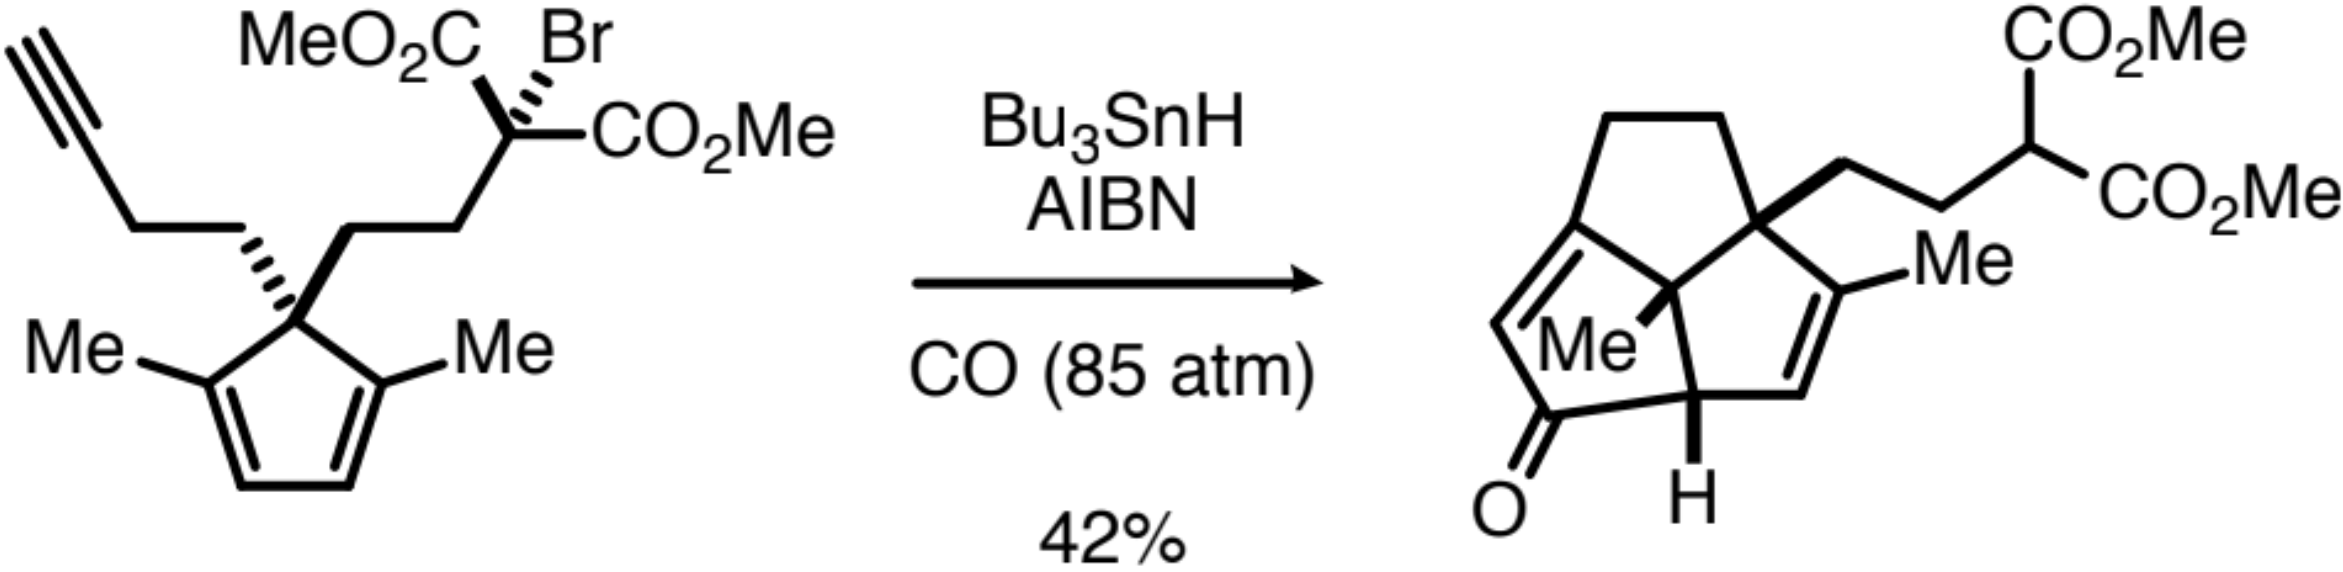
\includegraphics[width=0.55\linewidth]{PSet1Q1.png}
        \caption{PSet 1, Q1.}
        \label{fig:PSet1Q1}
    \end{figure}
    \item A \emph{key} technique for thinking about, rationalizing, and solving this problem is \textbf{bond dissociation energy} (BDE).
    \item In fact, we can apply BDE from the very beginning: AIBN's \ce{C-N} bond is the first to break because its BDE is an extremely low $\sim\SI{30}{\kilo\calorie\per\mole}$.
    \begin{itemize}
        \item Additionally, AIBN's \ce{C-N} bonds do not have to break symmetrically. Rather, one bond may break first (driven by its vibrational modes) to generate the stable tertiary carbon-centered radical \emph{and} a nitrogen radical.
        \item After some finite time (from picoseconds to much longer), the second \ce{C-N} bond will split, off-gassing \ce{N2}.
    \end{itemize}
    \item At this point, we must remember that this is a three-step radical reaction (initiation, propagation, termination), and AIBN is our initiator.
    \begin{itemize}
        \item Thus, we don't have \emph{equivalents} of AIBN to speak of, but rather a tiny amount in a sea of everything else.
    \end{itemize}
    \item Our AIBN radical is very stable, but the \ce{H-SnBu3} bond is so weak that it will still break when the two bump into each other.
    \item Indeed, BDE can justify why this bond breaks over any of the reactant \ce{C-H}'s.
    \begin{itemize}
        \item \ce{H3C-H} is $\SI{100}{\kilo\calorie\per\mole}$.
        \item \ce{HR2C-H} is $\sim\SI{90}{\kilo\calorie\per\mole}$.
        \item Tributyl tin hydride BDE is a whopping $\sim\SI{73}{\kilo\calorie\per\mole}$.
        \item Know BDEs!! \href{https://en.wikipedia.org/wiki/Carbon%E2%80%93hydrogen_bond#Reactions}{Here}'s a great resource for \ce{C-H} bonds on Wikipedia.
    \end{itemize}
    \item The \ce{*SnBu3} radical is halophilic, and does indeed head straight for the bromine to form a resonance-stabilized radical on the reactant.
    \begin{itemize}
        \item A typical \ce{C-Br} BDE is $\SI{68}{\kilo\calorie\per\mole}$.
        \item Why does AIBN pick off the \ce{H-SnBu3} over the bromine, then??
        \begin{itemize}
            \item Alexander M\"{u}ller suggested it could be because tin and bromine are closer on the periodic table that they preferentially react (think hard/soft acid base theory).
        \end{itemize}
    \end{itemize}
    \item Once we create the stabilized radical on the compound, we have to think about where it could go.
    \begin{itemize}
        \item Do a \ce{C-H} abstraction analysis to see what hydrogens the radical might be able to pick off.
        \item The methyl hydrogens are relatively accessible and allylic, but the transition state would be seven-membered, which is less than ideal. Same with the propargyl hydrogens.
        \item Indeed, 1,5-\ce{H} atom transfer is the most favorable because it's a six-membered transition state.
        \begin{itemize}
            \item Linear, intermolecular is the most stable transition state.
            \item But when we get to 1,5-abstraction, intermolecular concentration dependencies (think chelate effect) start to compete with linearity.
            \item However, 5-exo-trig is favorable addition chemistry.
            \begin{itemize}
                \item 6-endo-trig will be more stable thermodynamically (secondary radical formation).
                \item When 5-exo-trig is irreversible, we form that (the kinetic product).
                \item When 5-exo-trig is reversible, we form exclusively the 6-endo-trig product.
            \end{itemize}
            \item Look up Baldwin's Rules!!
            \begin{itemize}
                \item Exo/endo because the radical is outside/inside the formed ring.
                \item dig/trig/tet naming is due to the hybridization of the carbon we're attacking ($sp$, $sp^2$, $sp^3$ --- respectively).
            \end{itemize}
        \end{itemize}
        \item Be able to switch fluently between $\pKa$'s and BDEs.
        \begin{itemize}
            \item An $sp$ carbanion is more stable because we're holding that electron density tight near the positive nucleus.
            \item An $sp$ radical is extremely unstable because it has nowhere to draw electron density from.
            \item Hyperconjugation stabilizes a primary radical over the methyl radical.
            \item The AIBN radical is not stabilized by an EWG (EWGs destabilize radicals), but it is stabilized by resonance with the cyano group.
        \end{itemize}
    \end{itemize}
    \item So if hydrogen abstraction is less than ideal, let's think about what other kinds of chemistry radicals can do.
    \item Addition chemistry is one major such option! Double bonds are nucelophilic sites that a radical will naturally be attracted to, so our achiral compound can undergo a radical attack at either of the quaternary carbons with essentially the same effect.
    \begin{itemize}
        \item Thus, we will have a racemic mixture of products, but the stereochemistry of each molecule will be set by this attack.
        \item That's why Mo wanted the stereochemistry indicated; to show that the attack will lead to a syn product.
        \item Indeed, the \emph{cis}-fused 5-membered ring is \SI{15}{\kilo\calorie\per\mole} more stable than the \emph{trans} equivalent.
    \end{itemize}
    \item We can now resonate the radical over to the more stable tertiary position.
    \item Now we begin the abstraction analysis over again.
    \begin{itemize}
        \item No good-looking hydrogens to abstract, so it's probably addition chemistry again.
        \item If we add into the alkyne, we can do a kinetically favored 5-exo-dig.
        \item Additionally, there \emph{will} be a thermodynamic driving force for this reaction: Compare bond energies! A \ce{C-C} $\sigma$-bond is stronger than a \ce{C#C} $\pi$-bond.
    \end{itemize}
    \item Maxim: Whenever we have the opportunity to form a \ce{C-C} $\sigma$-bond, we like to do that.
    \item Now is a good time to pick up a CO.
    \begin{itemize}
        \item Again, we are thermodynamically driven by the breaking of a \ce{C#O} triple bond to form a \ce{C-C} single bond.
        \item How about the stereochemistry?
        \begin{itemize}
            \item We need the \emph{Z} alkene to complete the cyclization, but in fact, the \emph{Z} and \emph{E} alkenes are equivalent! This is because resonance with the radical allows unrestricted rotation around the "alkene" bond in the other resonance structure.
            \item Note that equilibrium arrows are good for E/Z isomerism because we are moving the atoms, not just the electron density as in resonance.
        \end{itemize}
    \end{itemize}
    \item The rate of cyclization of the acyl radical must outcompete reduction by the tin hydride.
    \item Then we can break a bond to form a more stable radical.
    \item Finally, we can react with tributyltin hydride in a propagation step.
    \item Altogether, the full solution to PSet 1, Q1 is on the next page.
    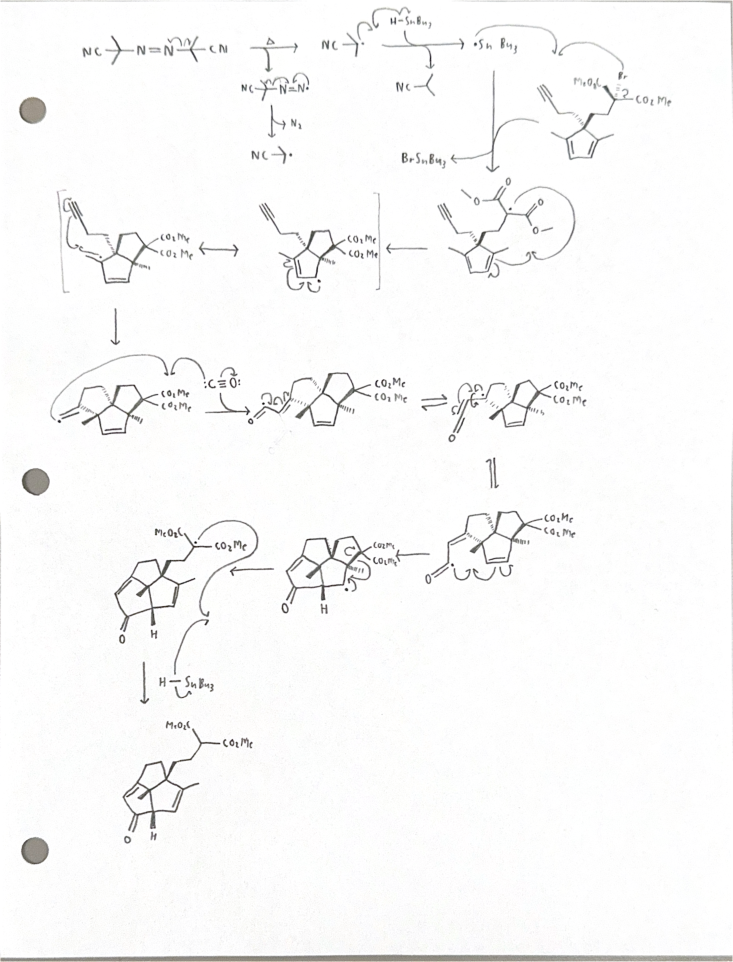
\includepdf{ExtFiles/PSet1Q1Full.pdf}
    \item We now begin discussing Problem 2.
    \begin{figure}[h!]
        \centering
        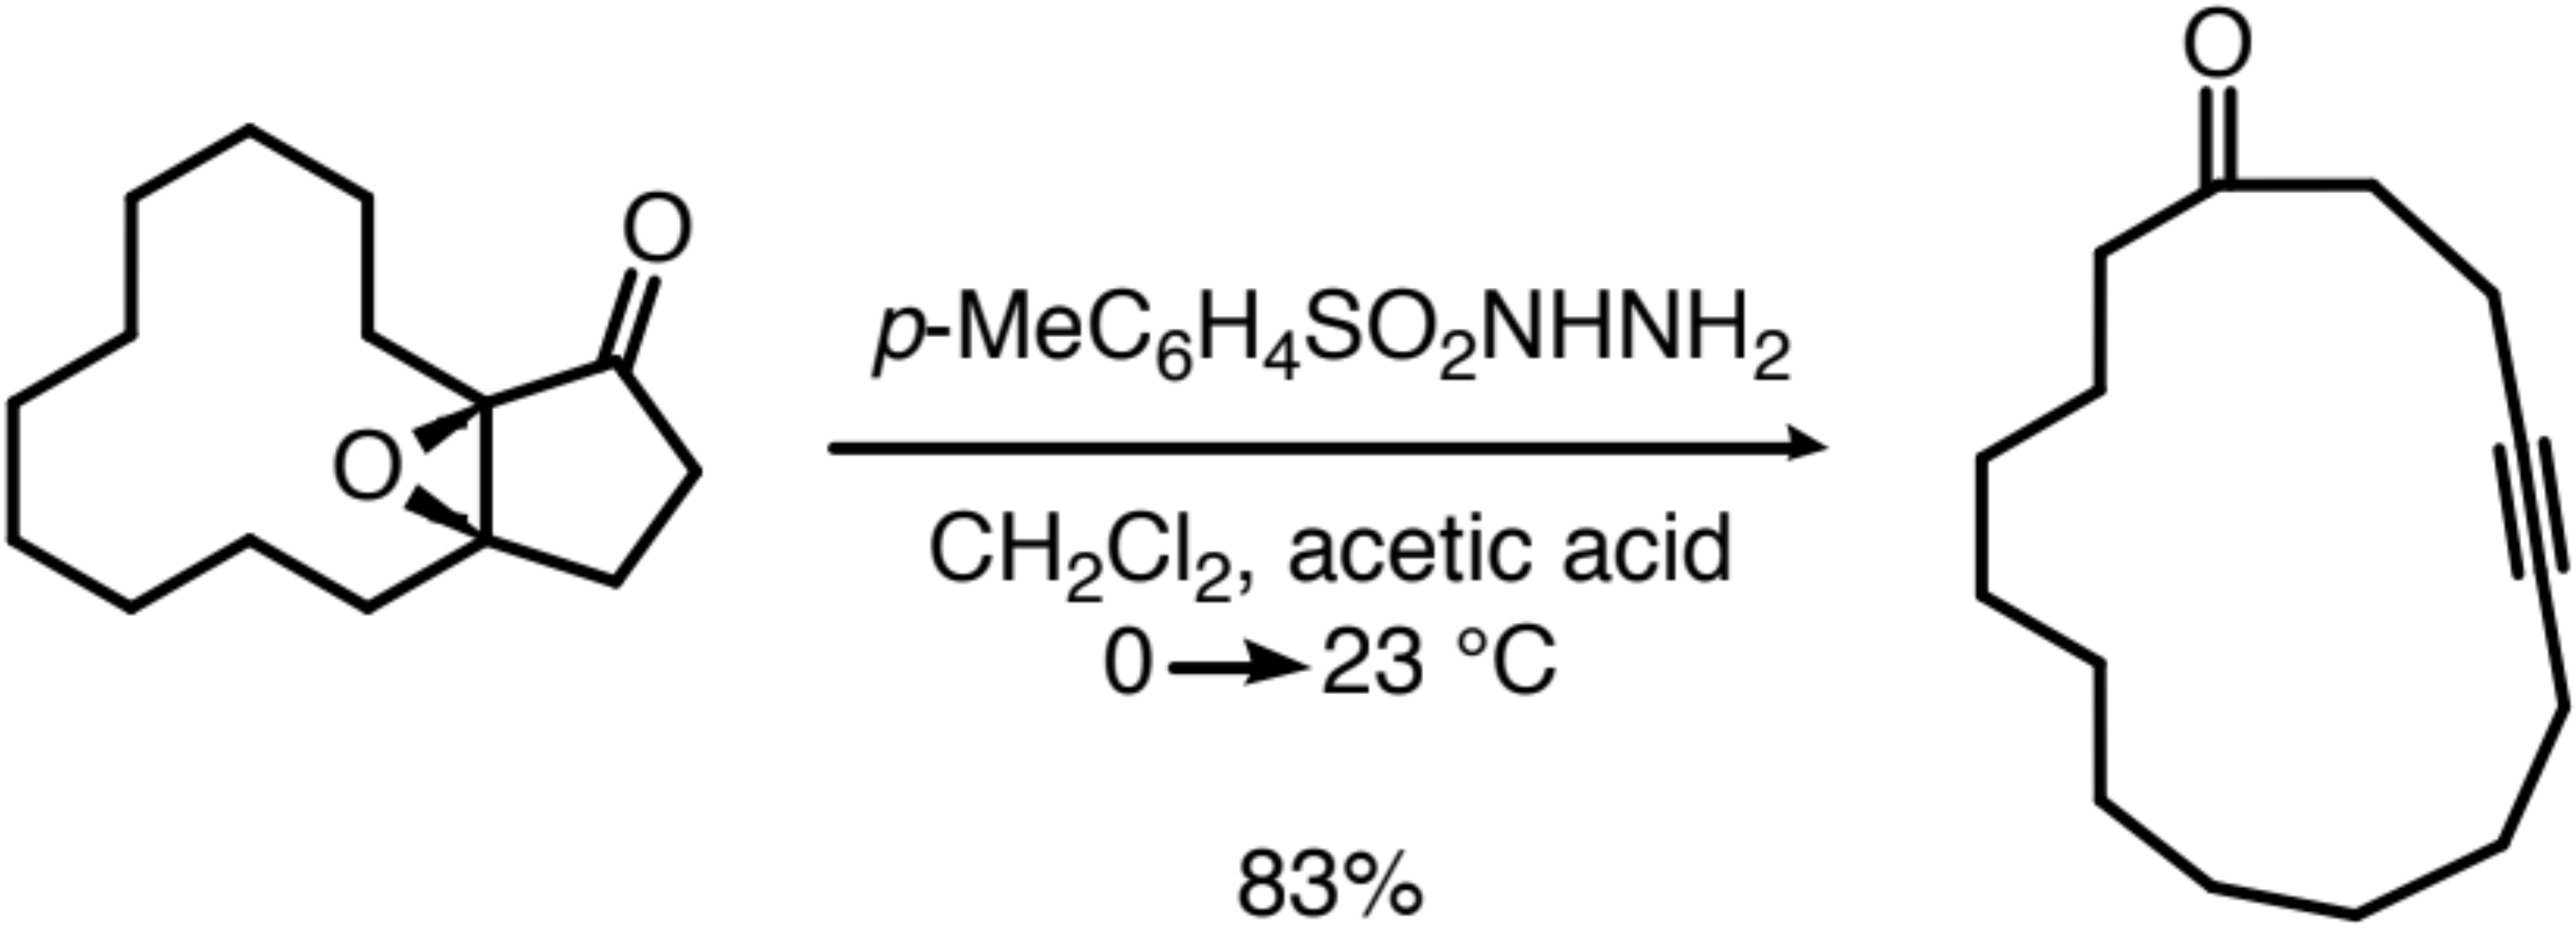
\includegraphics[width=0.5\linewidth]{PSet1Q2.png}
        \caption{PSet 1, Q2.}
        \label{fig:PSet1Q2}
    \end{figure}
    \item Aside: The naming of the reagent.
    \begin{figure}[h!]
        \centering
        \footnotesize
        \begin{subfigure}[b]{0.2\linewidth}
            \centering
            \chemfig{R-S(=[2]O)(=[6]O)-OH}
            \caption{Sulfonic acid.}
            \label{fig:sulfurOxidationa}
        \end{subfigure}
        \begin{subfigure}[b]{0.2\linewidth}
            \centering
            \chemfig{R-\charge{-90=\:}{S}(=[2]O)(=[6,,,,opacity=0]\phantom{O})-OH}
            \caption{Sulfinic acid.}
            \label{fig:sulfurOxidationb}
        \end{subfigure}
        \begin{subfigure}[b]{0.2\linewidth}
            \centering
            \chemfig{R-\charge{-90=\:,90=\:}{S}(=[6,,,,opacity=0]\phantom{O})-OH}
            \caption{Sulfenic acid.}
            \label{fig:sulfurOxidationc}
        \end{subfigure}
        \begin{subfigure}[b]{0.2\linewidth}
            \centering
            \chemfig{R-\charge{-90=\:,90=\:}{S}(=[6,,,,opacity=0]\phantom{O})-H}
            \caption{Thiol.}
            \label{fig:sulfurOxidationd}
        \end{subfigure}
        \caption{The oxidation states of sulfur.}
        \label{fig:sulfurOxidation}
    \end{figure}
    \begin{itemize}
        \item There are four different oxidation states of sulfur.
        \item They are referred to as (from most oxidized to most reduced) \textbf{sulfonic acid}, \textbf{sulfinic acid}, \textbf{sulfenic acid}, and \textbf{thiol}.
    \end{itemize}
    \item Now back to the problem at hand.
    \item In acidic solution, the first thing we can do is make the carbonyl more reactive via protonation.
    \begin{itemize}
        \item Note that the hydrazide may get protonated with the acid (and perhaps 90\% of it will be!), which would shut down nucleophilicity.
        \item But whatever hydrazide remains can do the demonstrated chemistry.
    \end{itemize}
    \item Then our hydrazine species can come in and add via nucleophilic addition.
    \item After this, we're fairly stable. But a negatively charged oxygen (like the epoxide) in acidic species can be protonated!
    \item After protonation, we'll want to break the epoxide ring. But where can we draw the electron density from?
    \begin{itemize}
        \item Looking around, notice that the second hydrazine nitrogen has a lone pair that can be used!
        \item Additionally, we can start building toward our alkyne located three carbons away from the position that could become the ketone after our new alcohol undergoes some modification.
    \end{itemize}
    \item Specifically, that modification will be kicking down the oxygen electrons to form the triple bond, kick out the leaving group, and break the leaving group in half all in one concerted step. This bond breaking process is still favorable because\dots
    \begin{itemize}
        \item The relevant orbitals align in an \textbf{antiperiplanar} fashion;
        \item We are strengthening and weakening consecutive bonds;
        \item Antibonding molecular orbitals receive donations of electron density, specifically the $\sigma^*$-antibonding orbital of the \ce{S-N} bond;
        \item The entropic gain in going from one molecule to three favors this step thermodynamically.
    \end{itemize}
    \item Aside: 4-membered transition states.
    \begin{figure}[H]
        \centering
        \footnotesize
        \schemestart
            \chemfig[atom sep=2.8em]{[:30]*6((-[:-100,0.7]!{wave})(-[:-140,0.7]!{wave})-[@{B1}]\charge{[extra sep=4pt]20=$\oplus$}{N}(-[:-40,0.7]H)(-[:-80,0.7]R)-[@{B2}]H-[@{B3},,,,opacity=0]O(-[,0.7]R)-[@{B4}]H-[@{B5},,,,opacity=0]HO-[@{B6}])}
        \schemestop
        \chemmove{
            \draw [curved arrow={2pt}{2pt}] (B6) to[bend right=40,looseness=1.2] (B5);
            \draw [curved arrow={2pt}{2pt}] (B4) to[bend right=40,looseness=1.2] (B3);
            \draw [curved arrow={2pt}{2pt}] (B2) to[bend right=40,looseness=1.2] (B1);
        }
        \caption{Using an acid as a proton transfer agent.}
        \label{fig:acidProtonTransfer}
    \end{figure}
    \begin{itemize}
        \item At a minimum, look to add an \ce{O-H} to the ring to make it a six-membered transition state.
        \item We could also do this in a two-step intermolecular process.
        \item As a specific example, amide bond hydrolysis under basic conditions is more reminiscent of the six-membered ring, though.
    \end{itemize}
    \item Aside: Protonation and $\pKa$'s.
    \begin{itemize}
        \item Ketones are much harder to protonate than comparable species.
        \begin{itemize}
            \item $\pKa$ of hydronium is $-1.7$.
            \item $\pKa$ of protonated ethylene oxide (the simplest epoxide) is $-2$.
            \item $\pKa$ of protonated carbonyl is $-6$ to $-8$.
        \end{itemize}
        \item Protonated THF is more easily stabilized by solvation effects than protonated diethyl ether because the "arms" are being held back in THF, so the oxygen lone pairs are more accessible.
        \item Carboxylic acid derivatives vary in terms of how hard they are to protonate.
        \begin{itemize}
            \item Acid chloride is $-9$.
            \item Amide is $0$ (resonance stabilization of the positive charge to the nitrogen).
            \item Ether is in the middle (still has resonance stabilization, but oxygen is more electronegative).
        \end{itemize}
    \end{itemize}
    \item Random note: Strain for a 5-membered ring is about \SI{5}{\kilo\calorie\per\mole}.
    \item Altogether, the full solution to PSet 1, Q2 is on the next page.
    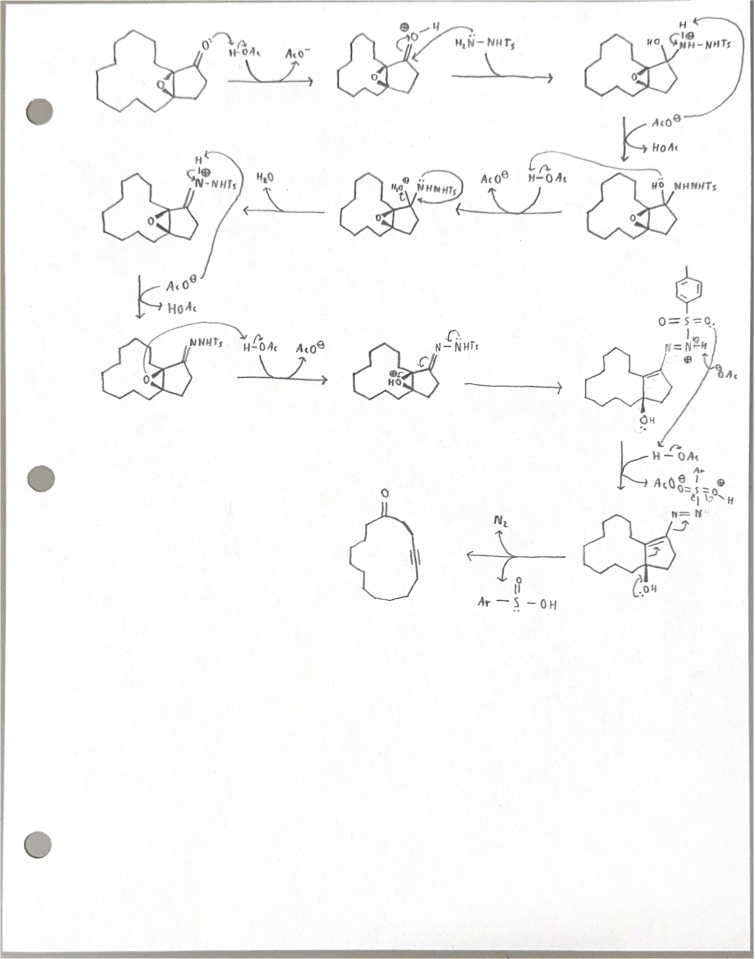
\includepdf{ExtFiles/PSet1Q2Full.pdf}
    \item We now begin discussing Problem 6.
    \begin{figure}[h!]
        \centering
        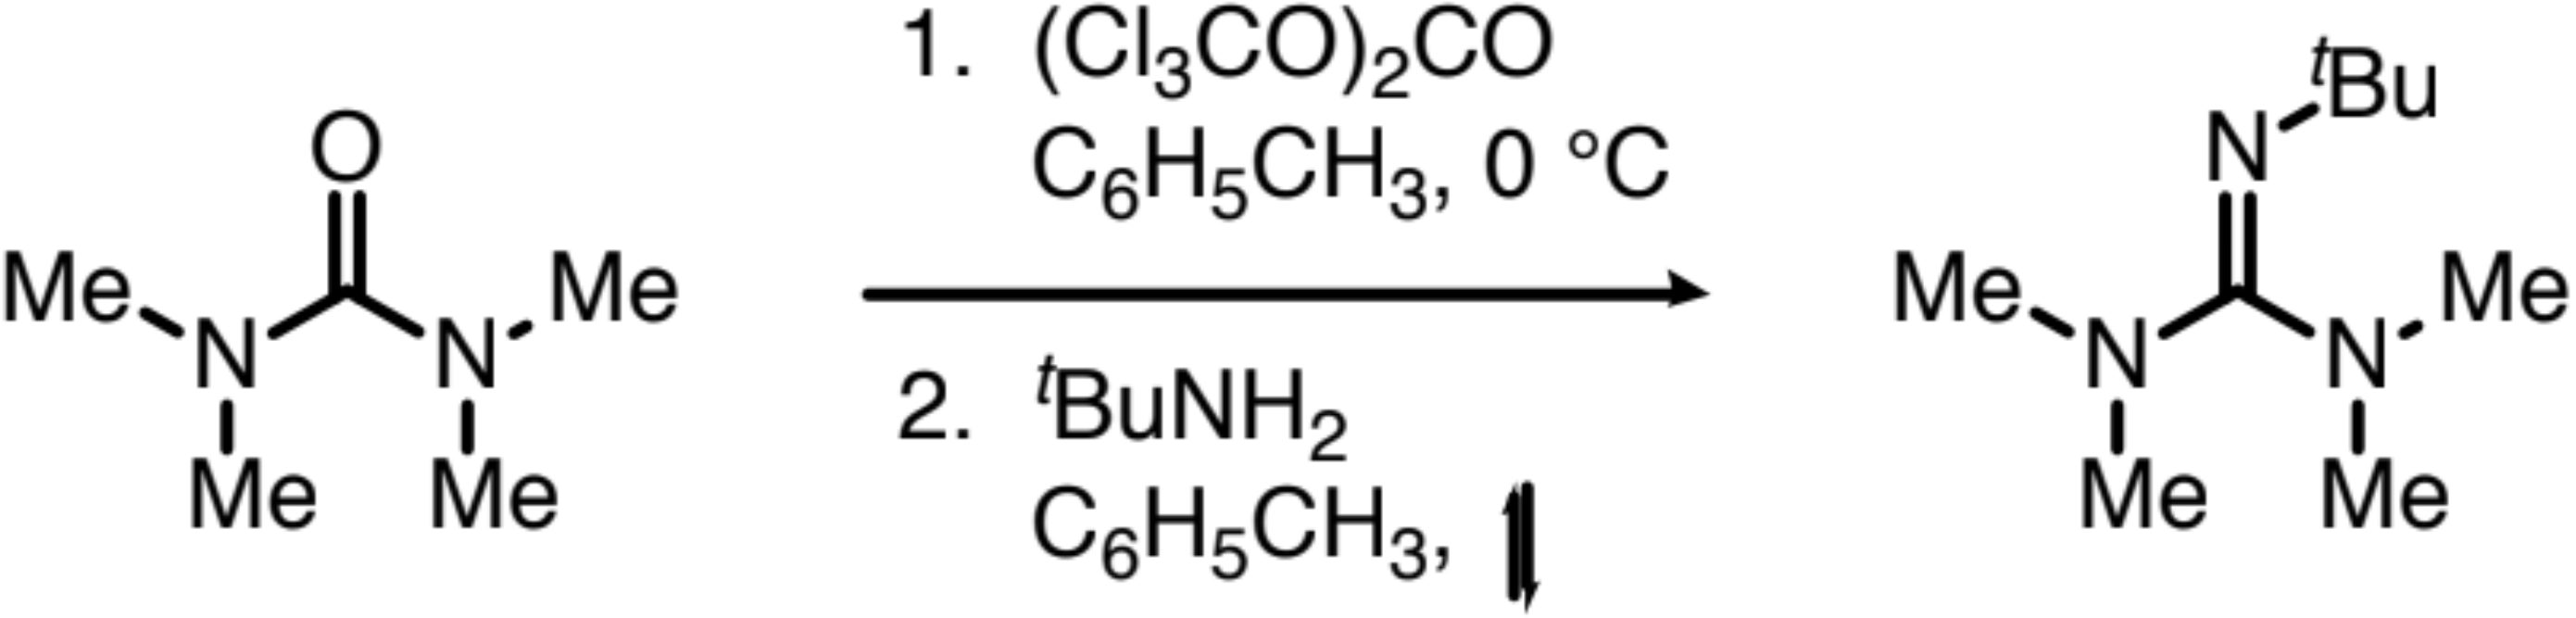
\includegraphics[width=0.5\linewidth]{PSet1Q6.png}
        \caption{PSet 1, Q6.}
        \label{fig:PSet1Q6}
    \end{figure}
    \item The first reagent is triphosgene. We use it because...
    \begin{itemize}
        \item It is far less toxic than phosgene;
        \item It generates phosgene \emph{in situ}.
    \end{itemize}
    \item First, make the reactant more nucleophilic via resonance.
    \item The reactant then attacks the reagent.
    \begin{itemize}
        \item Note that Mo is fine with us drawing out a nucleophilic substitution as electrons kicking up and back down in one step instead of in two (as Levin required). As such, I have done a bit of both in the final mechanism for this problem.
    \end{itemize}
    \item The leaving group is unstable, and undergoes $\alpha$-elimination of one chlorine.
    \item Chloride then attacks the positive center, kicking electrons up and down and kicking out a leaving group.
    \item \ce{CO2} then leaves, and we get another phosgene and chloiride.
    \item The chloride salt is where we end (the boxed intermediate in the final mechanism).
    \begin{itemize}
        \item Note that overall at this point, we've generated 2 equivalents of phosgene and 1 equivalent of \ce{CO2}; all chloride generated has been reincorporated into the molecule.
    \end{itemize}
    \item Now we add the second species.
    \item It attacks the iminium ion and kicks out the chloride.
    \item Chloride then neutralizes the molecule, generating \ce{HCl}.
    \item Finally, one more chloride attacks the remaining nitrogen hydrogen.
    \begin{itemize}
        \item Decide which way we go based on the $\pKa$'s of the relevant acids.
    \end{itemize}
    \item Note that we need one extra equivalent of \emph{tert}-butylamine to sequester the \ce{HCl}.
    \item Altogether, the full solution to PSet 1, Q6 is on the next page.
    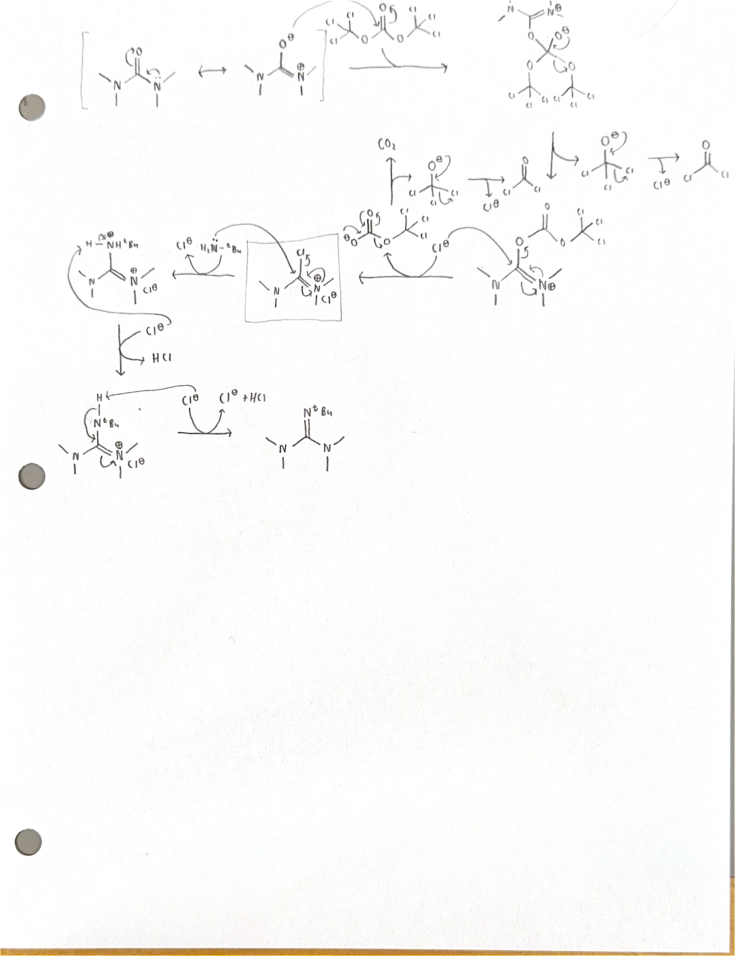
\includepdf{ExtFiles/PSet1Q6Full.pdf}
    \item Next time.
    \begin{itemize}
        \item We'll start next time with problems 4-5 of PSet 1.
        \item First 5 sessions are with Mo, then Alison has 6-10.
        \item 10 total sessions in this class.
    \end{itemize}
    \item Memorize more $\pKa$'s!!
\end{itemize}




\end{document}